
\documentclass[fleqn,addpoints]{exam}

\usepackage{units} 
\usepackage{graphicx}
\usepackage[fleqn]{amsmath}
\usepackage{cancel}
\usepackage{float}
\usepackage{mdwlist}
\usepackage{booktabs}
\usepackage{cancel}
\usepackage{polynom}
\usepackage{caption}
\usepackage{fullpage}
\usepackage{xfrac}
\usepackage{enumerate}

\everymath{\displaystyle}

% \printanswers

\ifprintanswers
  \usepackage{2in1, lscape}
\fi

\title{Math 141 Chapter Four Exam}
\date{July 17, 2013}
\author{}

\begin{document}

  \maketitle  

  \vspace{0.2in}
  \makebox[\textwidth]{Name:\enspace\hrulefill}
  \vspace{0.2in}

  \begin{center}
  \gradetable[h][pages]
  \bonusgradetable[h][pages]
  \end{center}

  \begin{questions}
    \uplevel{\section{Questions}}

    \question Write in logarithm form
      \begin{parts}
        \part[2] $2^3 = 8$

        \part[2] $e^x = y$
      \end{parts}

    \question Write in exponential form
      \begin{parts}
        \part[2] $\log_3 81 = 4$

        \part[2] $\ln x = 5$
      \end{parts}

    \question Evaluate each expression.
      \begin{parts}

        \part[2] $\log_8 64$

        \part[2] $\log 0.001$

        \part[2] $\log_7 \frac{1}{49}$

        \part[2] $\log_9 27$

        \part[2] $\log_8 16 + \log_8 32$

        \part[2] $\log_5 100 - \log_5 4$

      \end{parts}

    \question[5] solve for x:
      \[
        \log_x 27 = \frac{3}{2}
      \]

    \question[5] Simplify:
      \[
        \log \left( \frac{x^2y^3}{z} \right)
      \]

    \question Write as the sum/difference of logarithms:
      \begin{parts}
        \part[5]
          \[
            \ln \sqrt{ \frac{2x^3}{(x + 1)^3 (x - 2)^2} }
          \]

        \part[7]
          \[
            \ln \left[ \frac{ \sqrt{x + 2} \sqrt[3]{x - 1} }{ (x + 3)^4 } \right]
          \]

      \end{parts}

    \question[7] Write as a single logarithm:
      \begin{parts}
        \part[5]
          \[
            \ln (x + 2) + 2 \ln (x + 3) - \frac{1}{2} \ln x 
          \]

          \part[7]
          \[
            \log \sqrt{x - 1} + \log{x + 1} - 2 \log\left( x^2 + 1 \right)
          \]

      \end{parts}

      \begin{solution}
        \begin{align*}
          \ln (x + 2) + 2 \ln (x + 3) - \frac{1}{2} \ln x & = \ln (x + 2) + \ln (x + 3)^2 - \ln x^{1/2} \\
                                                          & = \ln \left[ (x + 2)(x + 3)^2 \right] - \sqrt{x} \\
                                                          & = \ln \frac{ (x + 2)(x + 3)^2 }{\sqrt{x}} \\
        \end{align*}
      \end{solution}

    \question[3] Write as a function of $\ln$ (change of base)
      \[
        \log_5 7
      \]

    \question $f(x) = 1 - 2^x$
      \begin{parts}
        \part[3] what is the range?

        \part[2] what is the y-intercept?

        \part[5] plot the graph
          \begin{solution}
            \begin{figure}[H]
              \centering
              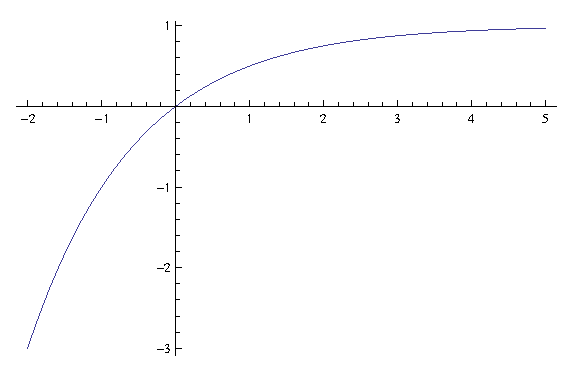
\includegraphics[scale=0.9]{graph_1.eps}
              \caption*{$f(x) = 1 - 2^x$}
            \end{figure}
          \end{solution}

      \end{parts}

    \question $f(x) = 3^{-x} + 2$
      \begin{parts}
        \part[3] what is the range?

        \part[2] what is the y-intercept?

        \part[5] plot the graph
          \begin{solution}
            \begin{figure}[H]
              \centering
              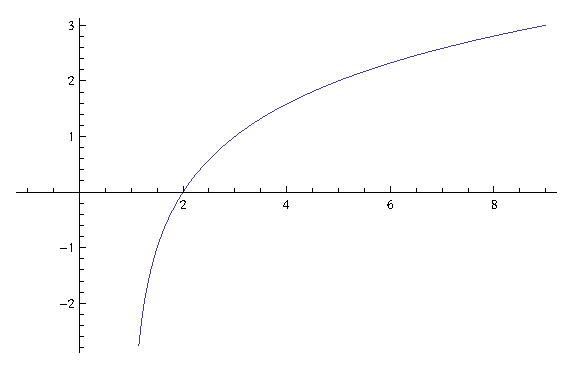
\includegraphics[scale=0.9]{graph_2.eps}
              \caption*{$f(x) = 3^{-x} + 2$}
            \end{figure}
          \end{solution}
      \end{parts}

    \question[5]
      If the magnitude of a sound is 85 dB, what is its intensity?  
      
      % If the intensity of the crowd sound at a Seahawks game is $I = \unit[1 \times 10^{-5}]{W/m^2}$, what is the
      % magnitude of the sound in decibels?

      \begin{solution}
        \begin{align*}
          M        & = 10 \log{I}{I_0} \\
          \\
          85       & = 10 \log \frac{I}{10^{-12}} \\
          8.5      & = \log \frac{I}{10^{-12}} \\
          10^{8.5} & = \frac{I}{10^{-12}} \\
          I        & = 10^{-3.5} \\
        \end{align*}
      \end{solution}


    \uplevel{\section{Extra Credit}}

    \bonusquestion[10]
      Multiply three consecutive integers together and then add the second integer to the product.  Use synthetic
      division to help prove that the sum is the cube of an integer and determine which integer.

      \begin{solution}
        If $x$ is the first number, the other two numbers are $x + 1$ and $x + 2$.  When you multiply the three
        numbers and add the second one, you get:
        \[
          x(x + 1)(x + 2) + (x + 1) = x^3 + 3x^2 + 3x + 1
        \]

        The only possible zeros are $x = \pm 1$.  If you try both of them, you find that $(x + 1)$ is the only
        factor and:
        \[
          x^3 + 3x^2 + 3x + 1 = (x + 1)^3
        \]

        Another way of seeing the same thing without doing any division is to factor $(x+1)$ out of the original
        equation and simplify:
        \begin{align*}
          x(x + 1)(x + 2) + (x + 1) &= (x+1) [ x(x+2) + 1 ] \\
                                    &= (x + 1) \left( x^2 + 2x + 1 \right) \\
                                    &= (x + 1) (x + 1)^2 \\
                                    &= (x + 1)^3 \\
        \end{align*}
        
      \end{solution}
  \end{questions}

\end{document}

